\chapter{COMMUNICATION \& AUTHENTICATION}\label{cha:auth} \index{authentication}
Since about all devices that are connected to a network are one way or another connected to the Internet you can bet that they find themselves in an untenanted or malicious environment. Everything connected to the Internet is very likely to be hacked. Thus, authentication is needed for remote sensing devices to communicate. \cite[]{auth:M2Mcom}\\
This chapter will present ways of authentication (two factor, M2M and biometric) that are in the area of this thesis. The section about biometric is included in the thesis because it has methods of measure strength of a biometric trait (especially fingerprint). These methods will be used when comparing strength of characteristic noise in the mobile device. \\


\section{Two factor authentication}\label{sec:2fauth} \index{two factor authentication}
There are more ways to authenticate a user than password, however it is the most common. There are three different types of authentication; 
\begin{itemize}
	\item Something the authenticator \textit{has} like a key, card, passport and so on
	\item Something the authenticator \textit{knows} for example password
	\item Something the authenticator \textit{is}, known as biometrics such as fingerprint or iris pattern
\end{itemize}
\cite[p.~31]{rosssec} \\
Authentication in two factor means a combination of two of the three types of authentication above. An example can be the use of a credit card (you have) in combination with a PIN-code (you know) to collect the money from an ATM. Something the authenticator has and knows is the most common combination. The biggest reason for that biometrics isn't that common yet is due to costs.
\cite[p.~47]{rosssec}

\section{Challenge-Response authentication}\label{sec:challResp} \index{challenge-response}
The challenge-response protocol is built upon the idea that the user of a system first must complete a challenge decided by the system in order to access the system. An example is modern car keys when trying to start the engine, the engine controller gives the key a challenge consisting of a random $n$-bit number. The key encrypts the challenge and responds. \\
The problem challenge-response protocols faces is often to achieve good randomness, thus if the challenge is not random enough there is a risk for a malicious user to calculate the $n$-bit number. \\
There are other applications than locks, like the HTTP Digest Authentication. That uses the authentication process where a web server challenges a client or a proxy with the common secret of a password. The server sends nonce to the client or proxy, that hash the nonce with the password and the requested URI. (Nonce is an arbitrary number that only can be used once, often generated as random or pseudo-random.)This authentication mechanism is not vulnerable to password snooping and is used in cases like client-server-authentication in SIP or the protocol for Voice-Over-IP telephony. This protocol is vulnerable to man-in-the-middle attacks. \\
\\
Ross states that a much more common use of challenge response is in \textit{two-factor authentication} (~\sectionref{sec:2fauth}). An example of use is if you have a bank card reader when accessing your bank on the Internet. When you want to log in there are a random set of $n$ numbers displayed in the screen. You put these numbers together with a PIN into your bank card reader. The reader encrypts these numbers (pin + $n$ numbers) using a secret key shard with the server of the bank. The first $n$ numbers of the encryption is displayed on the card reader and you enter this in the login screen as a password.
\newpage
\begin{figure}[h]
	\centering
    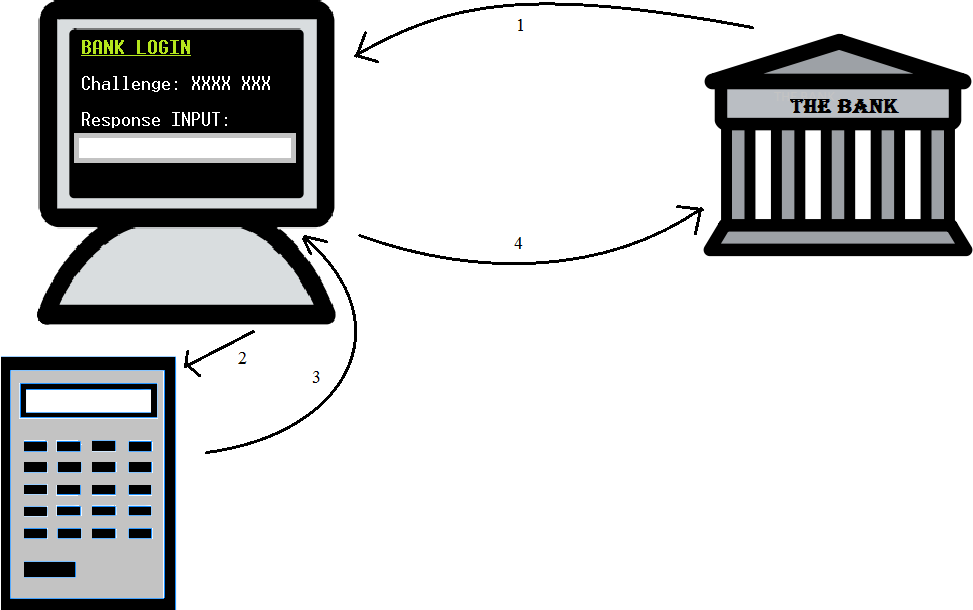
\includegraphics[scale=0.4]{img/challenge-response-bank}
    \caption{Challenge-response authentication with bank card reader}
  \label{fig:challengeResponse}
\end{figure}
Describe ~\figureref{fig:challengeResponse}:
\begin{enumerate}
	\item Bank sending challenge XXXX XXX to the requesting address.
	\item User enters PIN and XXX XXX in the bank card reader.
	\item The reader encrypts the PIN and number with a secret key shared with the bank. The first numbers of the encryption are displayed o the reader. ($YYYY YYY = {XXXX XXX, PIN}_k$) 
	\item The user enters the encrypted numbers YYYY YYY on the log in screen and sends it as a password to the bank.
\end{enumerate}
~\cite[ch.3]{rosssec}

\section{M2M\index{M2M} (Machine-to-machine)}\label{sec:m2mauth}
Information that is exchanged via a communication network between machines has to establish conditions for doing so, that is where M2M is used. M2M is often a short synonym for M2M communication, meaning the communication conditions between devices. M2M communication is only the communication made between machines without any human behind it. A mobile device interacting with a call center application is not M2M, because there is a human behind the mobile device calling. 
The reason for using mobile devices in this thesis, that is controlled by a human, is that they contain many sensors. These sensors can be found in other simpler devices where M2M communication can be applied.
\\
M2M often involves similar devices in the same M2M area network that are interacting with an application. This makes it possible for devices to access public networks as well, via a gateway or router. An example is the heating system in smart homes. 
The area of M2M are important to make these devises talk without a human behind. This affects the requirements on the applications and networks dealing with the devices. Characteristics of these devices are listed blow:
\begin{itemize}
	\item \textit{Multitude} - The part of IoT that not directly interacts with humans is the part growing the most. It is soon expected to be significant more than the ones which interact directly with humans. This will put more pressure on application and networks dealing with all devices.
	\item \textit{Variety} - The connected devices has requirements like data exchange rate, form factor, computing, or communication capabilities. M2M applications have to be built, in order to define and develop common enabling capabilities.
	\item \textit{Invisibility} -  Meaning that the device has virtually zero human control. The more invisibly the less likely for error caused by humans. 
	\item \textit{Criticality} - Devices that can harm humans like electrical errors. Therefore reliability is an important factor. 
	\item \textit{Intrusiveness} - Many of the increasing connected devices raise the privacy question like refrigerators, stoves, doors, etc.
\end{itemize}
All these devices with no human control is like told above very different, but many of them is similar in some ways, such that the functionality is limited, low-powered, embedded and have long life cycles. The fact that they often are embedded makes it hard to separate between M2M communication and machine-to-human or human-to-human communication.
\cite[p.~2-4]{m2mComm}

\subsection{Difference between M2M and IoT}\index{IoT}
The term Internet-of-Things meaning everything that is connected to the Internet. IoT are now in its starting pits and ready to start the race. Machine-to-machine communication is a part of that, but it also covers other areas and IoT some that M2M doesn't. 
% Måla en fin graf med två ringar som sitter ihop om du vill förklara.
The common denominator is according to Polsonetti the \textit{remote device access}, where the embedded hardware modules in a machine that communicate wireless or not is M2M applications. Remote device access for IoT has a wider perspective that not only including same device communication but also passive and other low-power sensors that not can be motivated as a M2M hardware module.
\cite[]{cpM2MIoT}

\subsection{M2M authentication}\index{M2M authentication}
There is no standardized way of authentication in M2M, but effort is done in the area. An example is authentication based on a machines fingerprint. (This fingerprint isn't of the same character as the one this thesis.)  The fingerprint in the example  consist of hardware message of computers, such serial number of CPU, MAC address of network card, Machine ID etc. \cite[]{auth:M2M} \\
These things have through the years been proven to be pretty easy to spoof. There are hundreds of blog-articles and forum topics of how to do that in many platforms like mobile devices. \\
\\
Quote about M2M authentication:
\begin{center} 
\textit{``\dots traditional methods such as “what you know and who you are” may not be applied''.}
\end{center}
\cite[]{auth:M2Mcom}
This quote states pretty well the aim of this thesis (section~\ref{sec:aim}). That is to use what the device is with biometric authentication that is more  tried and tested.


\section{The biometric process}\label{sec:biometric}\index{biometric process}
\begin{center}\textit{``A biometric system measures one or more behavioral characteristics...information of an individual to determine or verify his identity.''} \cite[p.~3]{introbio}\end{center}

\subsection{Recognition}
As said before is biometric something you \textit{are} and the person who wants to be recognized to the system. Buy, showing his or her biometric identifier (fingerprint, iris, DNA, etc.) to the biometric system, thus seen as a \textit{user} of the system. The strength in biometrics is also the fact that it knows if a user is known to the system even if the user denies it. \cite[ch.~1]{introbio}

\subsection{Biometric systems}\label{sec:bioSys}
There are some blocks for building a biometric systems, which can measure characteristics of a user. In biometrics these characteristics are called \textit{traits, indicators, identifiers, or modalities}, but in thesis it will still be called characteristics.\\
\\
The first step of biometric authentication is to collect biometric data and store it in a database with the user’s identity. The recognition is then done by again collecting biometric data from the user and compare to the database. This is the so called \textit{enrollment and recognition phase}. The raw biometric data is often destroyed after enrollment and the recognition is all about pattern matching. This matching is done in four steps;
\begin{enumerate}
	\item \textit{Sensor -} to collect the raw biometric samples, that can be an image, amplitude signal, online signature, odor or chemical-based.
	\item \textit{Feature extractor -} Makes the raw biometric samples comparable, mostly done in three pre-process operations; 
	\begin{itemize}
    	\item Quality assessment - Checks if the sample is good enough.
		\item Segmentation - removes the background noise from sample.
		\item Enhancement - Uses an algorithm to improve characteristic features of the sample.
    \end{itemize}
	\item \textit{Database -} that has the data from the enrollment phase together with some identity data (like name or ID). This database should having an access control mechanism for security reasons.
	\item \textit{Matcher -} where the sample from the enrollment is compared with the sample in recognition, to see if it's a match or not. This is done by having a match score to decide how close the enrolled and recognition sample is. The score is counted in different way depending on the characteristics that is used in the system. 
\end{enumerate}
\cite[ch.~1]{introbio}

\subsection{Biometric authentication}\index{biometric authentication}
Biometric authentication, is sometimes also called verification that answers the question \textit{Are you the one you say you are?}. There is also biometric identification that answers \textit{Are you someone known to the system?} but that is not what this thesis aims to answer. The practical difference between authentication and identification is that the user has to give the system some kind of information (username, passport, email etc.) on who they claim to be. But in identification the user just gives the sample to the system, which then checks if the user is known to the system or not. The identification look-up takes longer time since it compares the biometric input with all samples in the database, authentication only compare with the claimed identity. \cite[ch.~1]{introbio}

\subsection{Biometric measurements}\label{sec:bio:measure}
Biometric measurements are a bit trickier than in a password-based system where the answer just is match or not match. The accuracy of the biometric system must be considered when choosing characteristics. This is measured by two rates FRR\index{FRR} (False Reject Rate) that is the probability that two samples from the same user is not a match and FAR\index{FAR} (False Accept Rate) is the probability that two samples from different users is a match. 
There are a threshold $\eta$ that is used to decide the FRR and FAR. The proportion of authentic scores ($\omega_{1})$) that are less than $\eta$ is defined as FRR and the impostor score ($\omega_{0})$) that are greater than or equal to $\eta$ is FAR. The rates can be described mathematical as;
$$ FAR(\eta) = p(s\geq \eta | \omega_{0}) = \int_{\eta}^{\infty} p(s | \omega_{0}) ds, $$
$$ FRR(\eta) = p(s\geq \eta | \omega_{1}) = \int_{-\infty}^{\eta} p(s | \omega_{1}) ds, $$
where $p(s\geq \eta | \omega_{x})$ us the probability density function of the authentic respective impostor score. 
\cite[p.~18]{introbio}

\subsection{Design a biometric system}
When designing a biometric system it is done in an activity cycle of five steps. Depending on the outcome of one activity, the next step could be forward or redoing earlier activity. These five steps are explained below followed by an flow-chart of the design cycle.\\
\\
\textbf{Understand nature of application}\\
Deciding functionality upon type and classification based on how well the system fits this different behaviors; cooperative, overt, habituated users, attended, untenanted operation, controlled operation and open system. \\
The first is if the user will be \textit{cooperative} or not, like if the user wants to access something it is likely to cooperate. \textit{Overt} is if the user knows that it is object for biometric recognition. If the user interacts with the system a lot it is likely that the user will be \textit{habituated}. The enrollment and recognition operations can either be \textit{attended} by a human or not. The environment of the operations may have to be \textit{controlled} in terms of temperature, pressure, etc. in order to work. Last there is the question of if the system will be closed or \textit{open}, such if the database of biometric data will be shared between applications or be in one closed application.) \\
This chapter and the next that includes theory, can be compared to this part of the biometric design cycle.\\
\\
\textbf{Choose biometric characteristics }\label{auth:bio:character}\\ 
This choice is based on seven different factors. The disadvantages of biometrics is that it will never be completely solid, therefore factors will have different significance in different systems.
\begin{enumerate}
	\item \textit{Universality,} the fail-to-enrollment (FTE) rate should be low.\index{FTE}\index{universality}
	\item If the \textit{uniqueness} of the characteristics is high the rate of FAR will be low. \index{uniqueness}
	\item The characteristic should be high in terms of \textit{permanence} and not be changing significantly over time.\index{permanence}
	\item \textit{Measurability} from the user perspective in terms of collecting characteristics should be convenient.\index{measurability}
	\item The time of the authentication is measured in \textit{performance}.\index{performance}
	\item User should have a high \textit{acceptability} when presenting their characteristics to the system.\index{acceptability}
	\item \textit{Circumvention}, in terms of how easy it is to maliciously fake the characteristics.\index{circumvention}
\end{enumerate} 

\textbf{Collect biometric data}\\ 
Apart from the collecting also includes factors of time, cost and size of the equipment.\\
\\
\textbf{Choose features and matching algorithm}\\ 
A critical step since this is the heart of the system and has to bee done with a great deal of knowledge of the selected characteristics and the data extracted from it. \\
\\
\textbf{Evaluate the biometric system}\\ 
The evaluation is done by asking different questions. There is no framework for doing this and it has to account different perspective that require experts of different field such psychology, business, computer science and statistics. The proposed method is in three evaluation-stages technology, scenario and operational. \cite{introbio}
\index{biometric design cycle}
\begin{figure}[!ht]
	\begin{tikzpicture}[node distance=1.6cm]
	\node (start) [justtext] {Start};
	\node (understand) [process, below of=start] {Understand nature of application};
	\draw [arrow] (start) -- (understand);
		
	\node (choose) [process, below of=understand] {Choose biometric characteristics};
	\draw [arrow] (understand) -- (choose);
		
	\node (collect) [process, below of=choose] {Collect biometric data};
	\draw [arrow] (choose) -- (collect);
	\node (coll) [right of=collect, xshift=1.3cm] {};

	\node (algorithm) [process, below of=collect] {Choose features and matching algorithm};
	\draw [arrow] (collect) -- (algorithm);
	\node (alg) [right of=algorithm, xshift=1.3cm] {};

	\node (evaluate) [process, below of=algorithm] {Evaluate the biometric system};
	\draw [arrow] (algorithm) -- (evaluate);

	\node (end) [justtext, below of=evaluate] {End};
	\draw [arrow] (evaluate) -- (end);

	\node (req) [justtext, text=blue, left of=understand, xshift=-3cm, yshift=-1cm] {Performance requirements};
	\draw (understand) -| (req);
	\draw [->,>=stealth] (req) |- (evaluate);
		
	\node (knowledge) [justtext, text=red, left of=algorithm, xshift=-1.5cm] {Prior knowledge};

	\draw [arrow, draw=red, very thick] (knowledge) |- (algorithm);

	\draw [dashed] (evaluate) -| (alg);
	\draw [darrow, dashed] (alg) -- (algorithm);
	\draw [dashed] (alg) -- (coll);
	\draw [darrow] (coll) -- (collect);
	\draw [darrow] (coll) |- (choose);
\end{tikzpicture}
	\caption{\label{fig:biodesigncycle} The design cycle of a biometric system}
\end{figure}
